\documentclass{beamer}
\usetheme{Warsaw}
\usepackage{graphicx}
\usepackage{caption}
\usepackage{subcaption}
\usepackage{longtable}
\usepackage{listings}
\usepackage{color}
%% The amssymb package provides various useful mathematical symbols
\usepackage{amssymb}
%% The amsthm package provides extended theorem environments
\usepackage{amsthm} 
\usepackage{amsmath} 
\usepackage{tmadd,tmath}
\usepackage[mathcal]{euscript} 
\usepackage{color}
\usepackage{textcomp}
\usepackage{algorithm,algorithmic}
\definecolor{listinggray}{gray}{0.9}
\definecolor{lbcolor}{rgb}{0.9,0.9,0.9}
\lstset{
  backgroundcolor=\color{lbcolor},
  tabsize=4,
  rulecolor=,
  language=c++,
  basicstyle=\scriptsize,
  upquote=true,
  aboveskip={1.5\baselineskip},
  columns=fixed,
  showstringspaces=false,
  extendedchars=true,
  breaklines=true,
  prebreak =
  \raisebox{0ex}[0ex][0ex]{\ensuremath{\hookleftarrow}},
  frame=single,
  showtabs=false,
  showspaces=false,
  showstringspaces=false,
  identifierstyle=\ttfamily,
  keywordstyle=\color[rgb]{0,0,1},
  commentstyle=\color[rgb]{0.133,0.545,0.133},
  stringstyle=\color[rgb]{0.627,0.126,0.941},
}

%% colors
\setbeamercolor{boxheadcolor}{fg=white,bg=black}
\setbeamercolor{boxbodycolor}{fg=black,bg=white}

%% slide numbers

%%---------------------------------------------------------------------------%%
\author[Stuart Slattery]{Stuart Slattery, Thomas Evans, Steven
  Hamilton\\
  \bigskip
  \href{mailto:slatterysr@ornl.gov}{\texttt{slatterysr@ornl.gov}} \\
  \bigskip
  Oak Ridge National Laboratory}

\date{\today} 
\title[Multilevel Monte Carlo \hspace{1mm}
  \insertframenumber/\inserttotalframenumber]{A Multilevel Monte Carlo
  Method for Linear Systems}
\begin{document}
\maketitle

%%---------------------------------------------------------------------------%%
\begin{frame}{Hardware-Based Motivation}

  \begin{itemize}
  \item Modern hardware is moving in two directions (Kogge,2011):
    \begin{itemize}
    \item Lightweight machines
    \item Heterogeneous machines
    \item Both characterized by low power and high concurrency
    \end{itemize}
    \medskip \medskip
  \item Some issues:
    \begin{itemize}
    \item Higher potential for both soft and hard failures (DOE,2012)
    \item Memory restrictions are expected with a continued decrease
      in memory/FLOPS
    \end{itemize}
    \medskip \medskip
  \item Potential resolution from Monte Carlo:
    \begin{itemize}
    \item Soft failures buried within the tally variance
    \item Hard failures mitigated by replication
    \item Memory savings over conventional methods
    \end{itemize}
  \end{itemize}

\end{frame}

%%---------------------------------------------------------------------------%%
\begin{frame}{Monte Carlo Methods for Discrete Linear Systems}

  \begin{itemize}
  \item First proposed by J. Von Neumann and S.M. Ulam in the 1940's
    \medskip \medskip
  \item Earliest published reference in 1950 (Forsythe,1950)
    \medskip \medskip
  \item General lack of publications on applications
    \medskip \medskip
  \item Plagued by slow convergence $\approx \frac{1}{\sqrt{N}}$
    \medskip \medskip
  \item Modern work yielded new applications (Evans,2009) (Evans,2013)
  \end{itemize}

\end{frame}

%%---------------------------------------------------------------------------%%
\begin{frame}{Monte Carlo Synthetic-Acceleration}

  \begin{beamerboxesrounded}[upper=boxheadcolor,lower=boxbodycolor,shadow=true]
    {MCSA Iteration}

    \[
    \ve{r}^{k} = \ve{b} - \ve{A}\ve{x}^{k}
    \]
    \[
    \ve{x}^{k+1/2} = \ve{x}^k + \ve{r}^k
    \]
    \[
    \ve{r}^{k+1/2} = \ve{b} - \ve{A}\ve{x}^{k+1/2}
    \]
    \[
    \hat{\ve{A}}\delta\ve{x}^{k+1/2} = \ve{r}^{k+1/2}
    \]
    \[
    \ve{x}^{k+1} = \ve{x}^{k+1/2} + \delta \ve{x}^{k+1/2}
    \]

  \end{beamerboxesrounded}

  \medskip \medskip
  \begin{itemize}
  \item Neumann-Ulam methods bound by the Central Limit Theorem
  \item Build on Sequential Monte Carlo method (Halton,1962)
  \item Neumann-Ulam Monte Carlo solver computes the correction
  \item Decouples MC error from solution error, exponential convergence
  \end{itemize}

\end{frame}

%%---------------------------------------------------------------------------%%
\begin{frame}{Monte Carlo Linear Solver Preliminaries}

  \begin{itemize}
  \item Split the linear operator
  \end{itemize}

  \[
  \ve{A}\ve{x} = \ve{b} \ \ \ \rightarrow \ \ \ \ve{x} = \ve{H} \ve{x}
  + \ve{b}
  \]

  \[
  \ve{H} = \ve{I} - \ve{A}
  \]

  \medskip
  \begin{itemize}
  \item Generate the \textit{Neumann series}
  \end{itemize}
  
  \[
  \ve{A}^{-1} = (\ve{I}-\ve{H})^{-1} = \sum_{k=0}^{\infty} \ve{H}^k
  \]

  \medskip
  \begin{itemize}
  \item Require $\rho(\ve{H}) < 1$ for convergence
  \end{itemize}

  \[
  \ve{A}^{-1}\ve{b} = \sum_{k=0}^{\infty} \ve{H}^k\ve{b} = \ve{x}
  \]

\end{frame}

%%---------------------------------------------------------------------------%%
\begin{frame}{Monte Carlo Linear Solver Preliminaries}

  \begin{itemize}
  \item Expand the Neumann series
  \end{itemize}

  \[
  x_i = \sum_{k=0}^{\infty}\sum_{i_1}^{N}\sum_{i_2}^{N}\ldots
  \sum_{i_k}^{N}h_{i,i_1}h_{i_1,i_2}\ldots h_{i_{k-1},i_k}b_{i_k}
  \]

  \begin{itemize}
  \item Define a sequence of state transitions
  \end{itemize}
  
  \[
  \nu = i \rightarrow i_1 \rightarrow \cdots \rightarrow i_{k-1}
  \rightarrow i_{k}
  \]

  \medskip
  \begin{itemize}
  \item Define the \textit{Neumann-Ulam decomposition}\footnote{The
    Hadamard product $\ve{A} = \ve{B} \circ \ve{C}$ is defined
    element-wise as $a_{ij} = b_{ij} c_{ij}$.}
  \end{itemize}

  \[
  \ve{H} = \ve{P} \circ \ve{W}
  \]

\end{frame}

%%---------------------------------------------------------------------------%%
\begin{frame}{Direct Method}

  \begin{itemize}
  \item Compute row-normalized transition probabilities and weights
  \end{itemize}

  \[
  p_{ij} = \frac{|h_{ij}|}{\sum_j |h_{ij}|},\ w_{ij} =
  \frac{h_{ij}}{p_{ij}}
  \]

  \medskip \medskip
  \begin{itemize}
  \item Generate an expectation value for the solution
  \end{itemize}

  \[
  W_{m} = w_{i,i_1} w_{i_1,i_2} \cdots w_{i_{m-1},i_m}
  \]
  \[
  X_{i=i_0}(\nu) = \sum_{m=0}^k W_{m} b_{i_m}
  \]
\end{frame}

%%---------------------------------------------------------------------------%%
\begin{frame}{Direct Method}

  \begin{itemize}
  \item Compute the probability of a particular random walk
    permutation
  \end{itemize}

  \[
  P(\nu) = p_{i,i_1} p_{i_1,i_2} \cdots p_{i_{k-1},i_k}
  \]

  \begin{itemize}
  \item Generate the estimator
  \end{itemize}

  \[
  E\{X(i_0 = i)\} = \sum_{\nu} P(\nu) X(\nu)
  \]

  \begin{itemize}
  \item Check that we recover the exact solution
  \end{itemize}
  
  {\small
  \[
  \begin{split}
    E\{X(i_0 = i)\}
    &=\sum_{k=0}^{\infty}\sum_{i_1}^{N}\sum_{i_2}^{N}\ldots
    \sum_{i_k}^{N} p_{i,i_1}p_{i_1,i_2}\ldots p_{i_{k-1},i_k}
    w_{i,i_1}w_{i_1,i_2}\ldots w_{i_{k-1},i_k} b_{i_k}\\ &= x_i
  \end{split}
  \]
  }

\end{frame}

%%---------------------------------------------------------------------------%%
\begin{frame}{Evolution of a Solution}

  \begin{figure}[htpb!]
    \begin{center}
      \scalebox{1.0}{ \input{heat_eq_setup.pdftex_t} }
    \end{center}
    \caption{\textbf{Heat Equation.}
      \textit{Distributed source of 1.0 in the domain.}}
  \end{figure}

\end{frame}

%%---------------------------------------------------------------------------%%
\begin{frame}{Evolution of a Solution: Direct Method}

  \begin{figure}[h!]
    \begin{center}
      \includegraphics<1>[width=4in]{direct_1.png}
      \includegraphics<2>[width=4in]{direct_10.png}
      \includegraphics<3>[width=4in]{direct_100.png}
      \includegraphics<4>[width=4in]{direct_1000.png}
    \end{center}
    \caption{
      \only<1>{\textbf{Direct solution to heat equation.}
        \textit{\sn{1}{0} total histories.} }
      \only<2>{\textbf{Direct solution to heat equation.}
        \textit{\sn{1}{1} total histories.} }
      \only<3>{\textbf{Direct solution to heat equation.}
        \textit{\sn{1}{2} total histories.} }
      \only<4>{\textbf{Direct solution to heat equation.}
        \textit{\sn{1}{3} total histories.} }
    }
  \end{figure}

\end{frame}

%%---------------------------------------------------------------------------%%
\begin{frame}{Adjoint Method}

  \begin{itemize}
  \item Solve the adjoint linear system
  \end{itemize}

  \[
  \ve{A}^T \ve{y} = \ve{d}
  \]

  \[
  \ve{y} = \ve{H}^T \ve{y} + \ve{d}
  \]

  \medskip
  \begin{itemize}
  \item Set the adjoint constraint
  \end{itemize}

  \[
  \langle \ve{A}^T \ve{x}, \ve{y} \rangle = \langle \ve{x}, \ve{A}
  \ve{y} \rangle
  \]

  \[
  \langle \ve{x}, \ve{d} \rangle = \langle \ve{y}, \ve{b} \rangle
  \]
  
\end{frame}

%%---------------------------------------------------------------------------%%
\begin{frame}{Adjoint Method}

  \begin{itemize}
  \item Generate the Neumann series for the adjoint operator
  \end{itemize}

  \[
  \ve{y} = (\ve{I} - \ve{H}^T)^{-1} \ve{d} = \sum_{k=0}^{\infty}
  (\ve{H}^T)^k\ve{d}
  \]

  \medskip
  \begin{itemize}
  \item Expand the series
  \end{itemize}

  \[
  y_i = \sum_{k=0}^{\infty}\sum_{i_1}^{N}\sum_{i_2}^{N}\ldots
  \sum_{i_k}^{N}h_{i_k,i_{k-1}}\ldots h_{i_2,i_1} h_{i_1,i} d_{i_k}
  \]

  \medskip
  \begin{itemize}
  \item Pick another constraint to yield the original solution
  \end{itemize}

  \[
  \ve{d} = \boldsymbol{\delta}_i,\ \langle \ve{y}, \ve{b} \rangle =
  \langle \ve{x}, \boldsymbol{\delta}_i \rangle = x_i
  \]
  
\end{frame}

%%---------------------------------------------------------------------------%%
\begin{frame}{Adjoint Method}

  \begin{itemize}
  \item Use the adjoint Neumann-Ulam decomposition
  \end{itemize}

  \[
  \ve{H}^{T} = \ve{P} \circ \ve{W}
  \]

  \[
  p_{ij} = \frac{|h_{ji}|}{\sum_j |h_{ji}|},\ w_{ij} =
  \frac{h_{ji}}{p_{ij}}
  \]

  \medskip
  \begin{itemize}
  \item Build the estimator and expectation value
  \end{itemize}

  \[
  X_j(\nu) = \sum_{m=0}^k W_{m} \delta_{i_m,j}
  \]

  \[
  \begin{split}
    E\{X_j\} &=\sum_{k=0}^{\infty}\sum_{i_1}^{N}\sum_{i_2}^{N}\ldots
    \sum_{i_k}^{N} b_{i_0} h_{i_0,i_1}h_{i_1,i_2}\ldots h_{i_{k-1},i_k}
    \delta_{i_k,j} \\ &= x_{j}
  \end{split}
  \]

\end{frame}

%%---------------------------------------------------------------------------%%
\begin{frame}{Evolution of a Solution: Adjoint Method}

  \begin{figure}[h!]
    \begin{center}
      \includegraphics<1>[width=4in]{adjoint_1.png}
      \includegraphics<2>[width=4in]{adjoint_10.png}
      \includegraphics<3>[width=4in]{adjoint_100.png}
      \includegraphics<4>[width=4in]{adjoint_1000.png}
      \includegraphics<5>[width=4in]{adjoint_10000.png}
      \includegraphics<6>[width=4in]{adjoint_100000.png}
      \includegraphics<7>[width=4in]{adjoint_1000000.png}
      \includegraphics<8>[width=4in]{adjoint_10000000.png}
    \end{center}
    \caption{
      \only<1>{\textbf{Adjoint solution to heat equation.}
        \textit{\sn{1}{0} total histories.} }
      \only<2>{\textbf{Adjoint solution to heat equation.}
        \textit{\sn{1}{1} total histories.} }
      \only<3>{\textbf{Adjoint solution to heat equation.}
        \textit{\sn{1}{2} total histories.} }
      \only<4>{\textbf{Adjoint solution to heat equation.}
        \textit{\sn{1}{3} total histories.} }
      \only<5>{\textbf{Adjoint solution to heat equation.}
        \textit{\sn{1}{4} total histories.} }
      \only<6>{\textbf{Adjoint solution to heat equation.}
        \textit{\sn{1}{5} total histories.} }
      \only<7>{\textbf{Adjoint solution to heat equation.}
        \textit{\sn{1}{6} total histories.} }
      \only<8>{\textbf{Adjoint solution to heat equation.}
        \textit{\sn{1}{7} total histories.} } 
    }
  \end{figure}

\end{frame}

%%---------------------------------------------------------------------------%%
\begin{frame}{Model Problem}

  Choose a simple homogeneous problem with Dirichlet conditions:
  \[
  \nabla^2 x = 0, \ \ve{x}_1 = 0,\ \ \ve{x}_N = 0
  \]

  Second order finite difference:
  \[
  (\nabla \ve{u})_i = \frac{\ve{u}_{i-1} - 2 \ve{u}_{i} + \ve{u}_{i+1}}{h^2}
  \]

  Monte Carlo requires $\rho(\ve{H}) < 1$ - scale by the diagonal:
  \[
  \ve{M}^{-1}\ve{A}\ve{x} = \ve{0}
  \]

  Choose initial guess to be some Fourier mode
  \[
  \ve{x}^0_i = \sin\Bigg( \frac{ik\pi}{N} \Bigg)
  \]

\end{frame}

%%---------------------------------------------------------------------------%%
\begin{frame}{Error Analysis}

  \begin{columns}

    \begin{column}{0.5\textwidth}
      \begin{figure}[h!]
        \begin{center}
          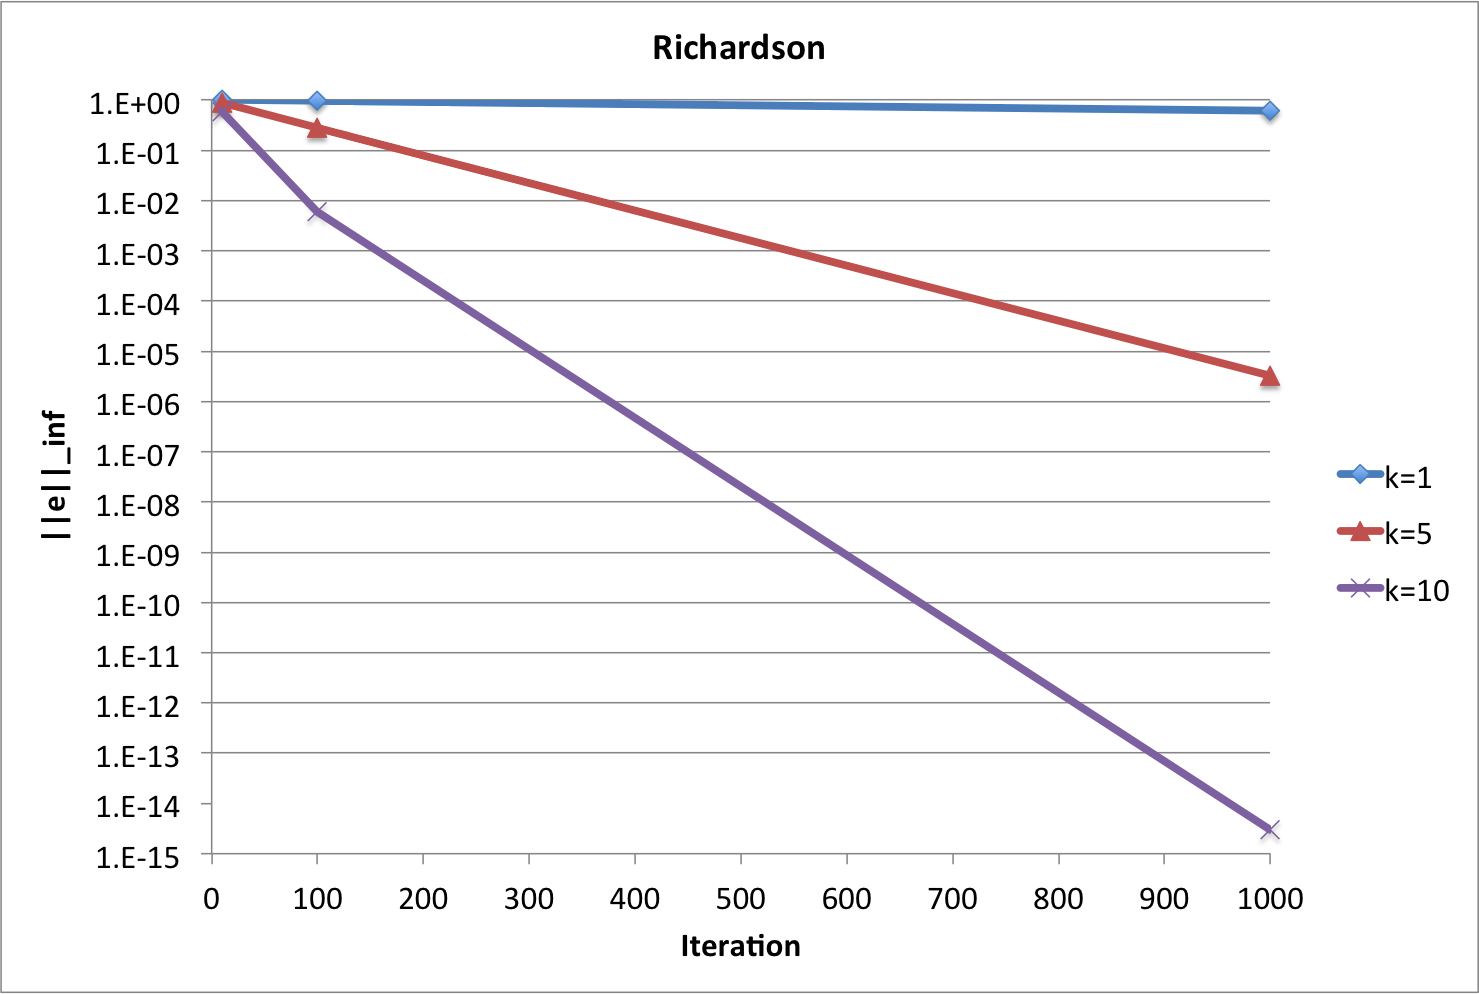
\includegraphics[width=2in]{richardson.png}
        \end{center}
        \caption{\textbf{Convergence of Richardson's iteration.}
          \textit{Better for larger wave numbers.}}
        \label{fig:richardson}
      \end{figure}
    \end{column}

    \begin{column}{0.5\textwidth}
      \begin{figure}[h!]
        \begin{center}
          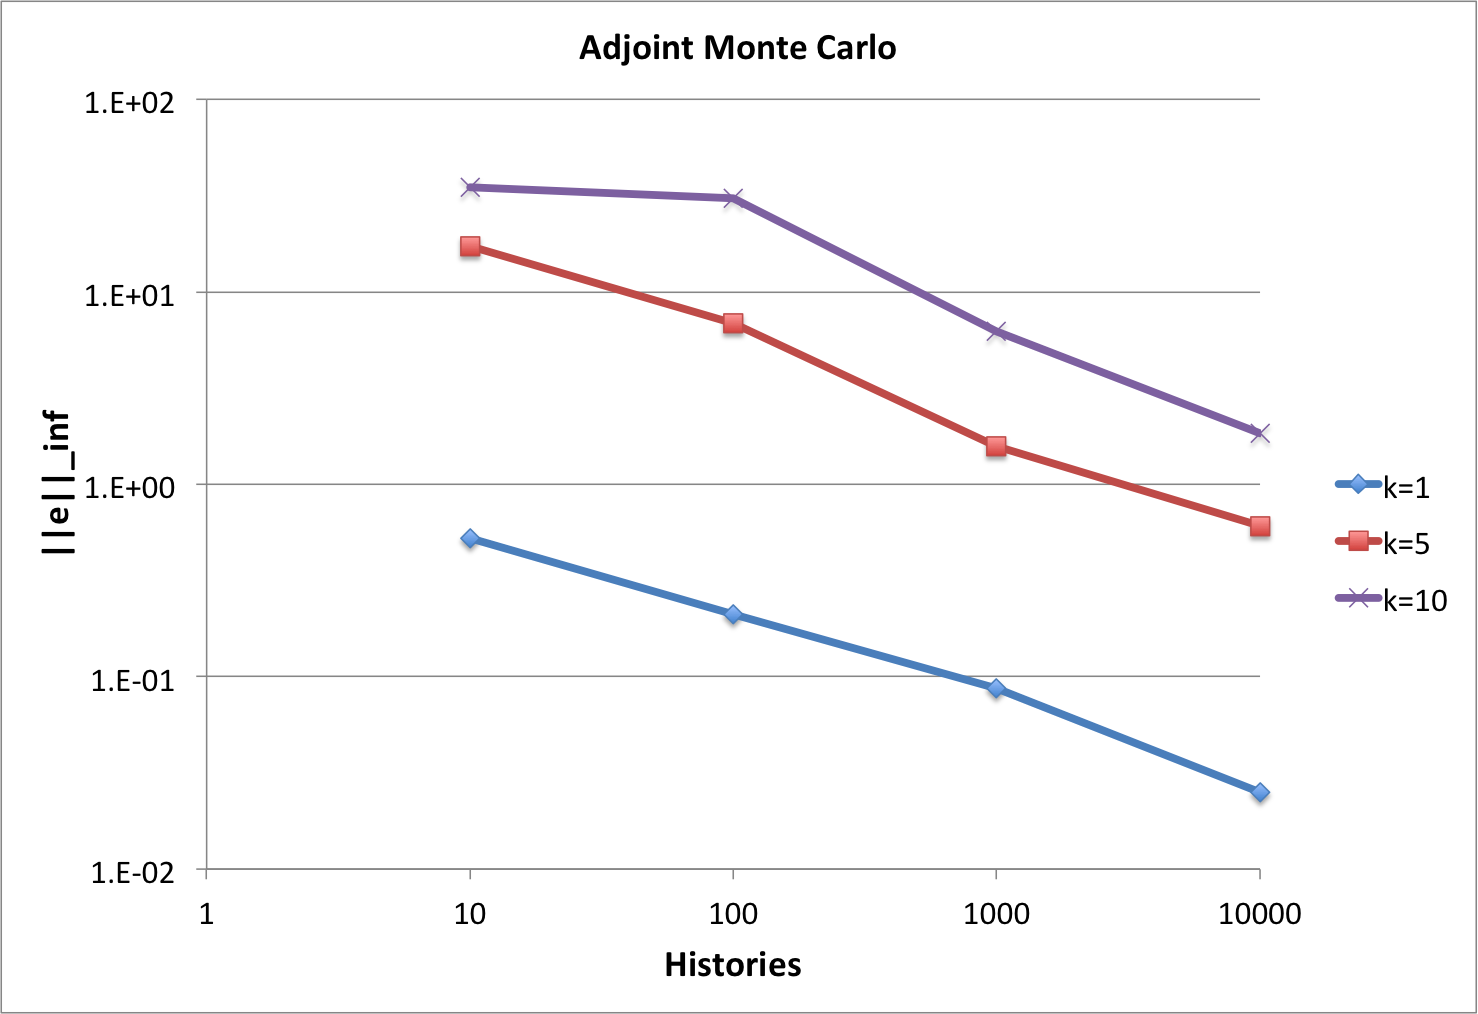
\includegraphics[width=2in]{adjoint_mc.png}
        \end{center}
        \caption{\textbf{Convergence of the adjoint Monte Carlo
            method.} \textit{Better for smaller wave numbers.} }
        \label{fig:adjoint_mc}
      \end{figure}
    \end{column}

  \end{columns}

  \begin{itemize}
    \item A multilevel scheme means larger errors at coarser levels
    \item More samples required at the coarser levels
    \item Potential reduction in run time if the coarse level problems
      are fast
  \end{itemize}

\end{frame}

%%---------------------------------------------------------------------------%%
\begin{frame}{Error Analysis}

  \begin{columns}

    \begin{column}{0.3\textwidth}

      \begin{figure}[h!]
        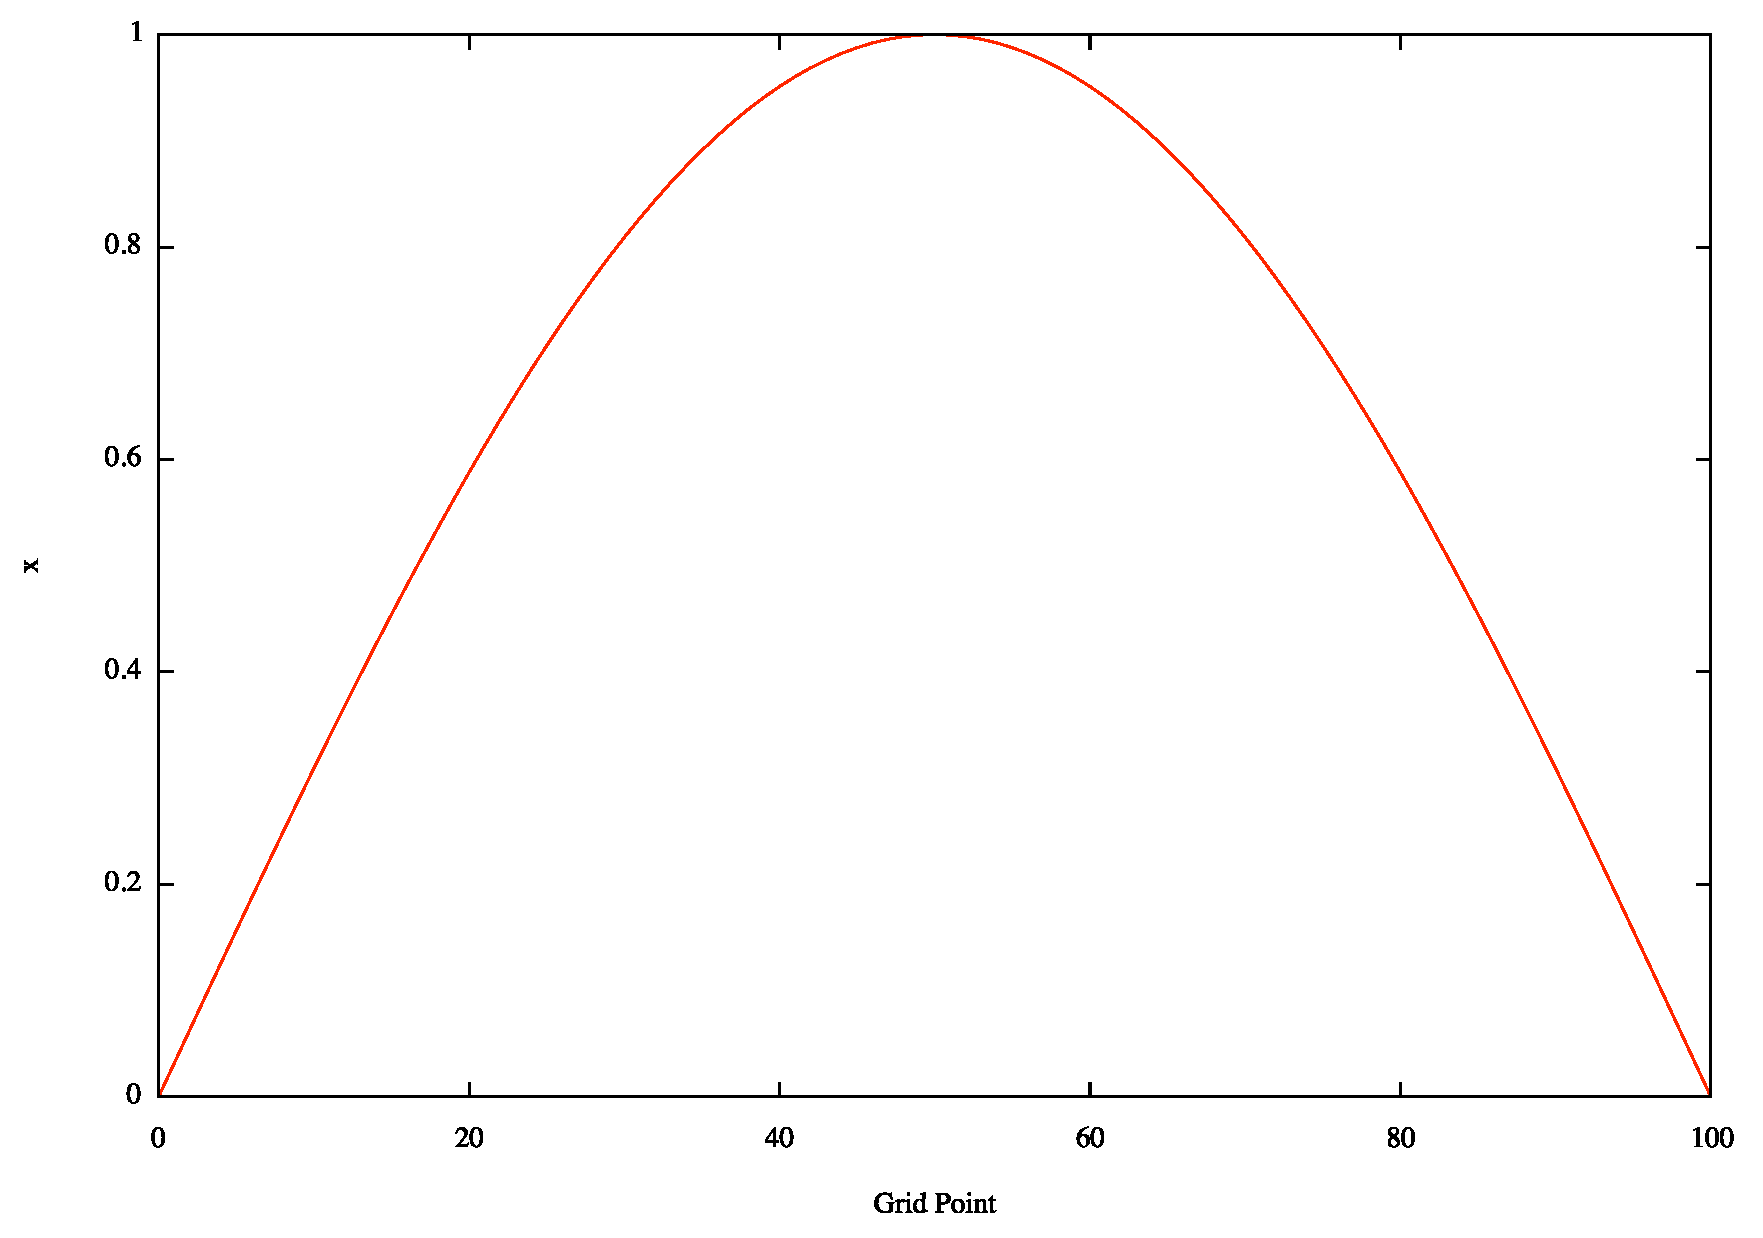
\includegraphics[width=1.5in]{mode_1.pdf}
        \caption{\textbf{$k = 1$.}}
      \end{figure}
      
     \vspace{-0.5in}

      \begin{figure}[b]
        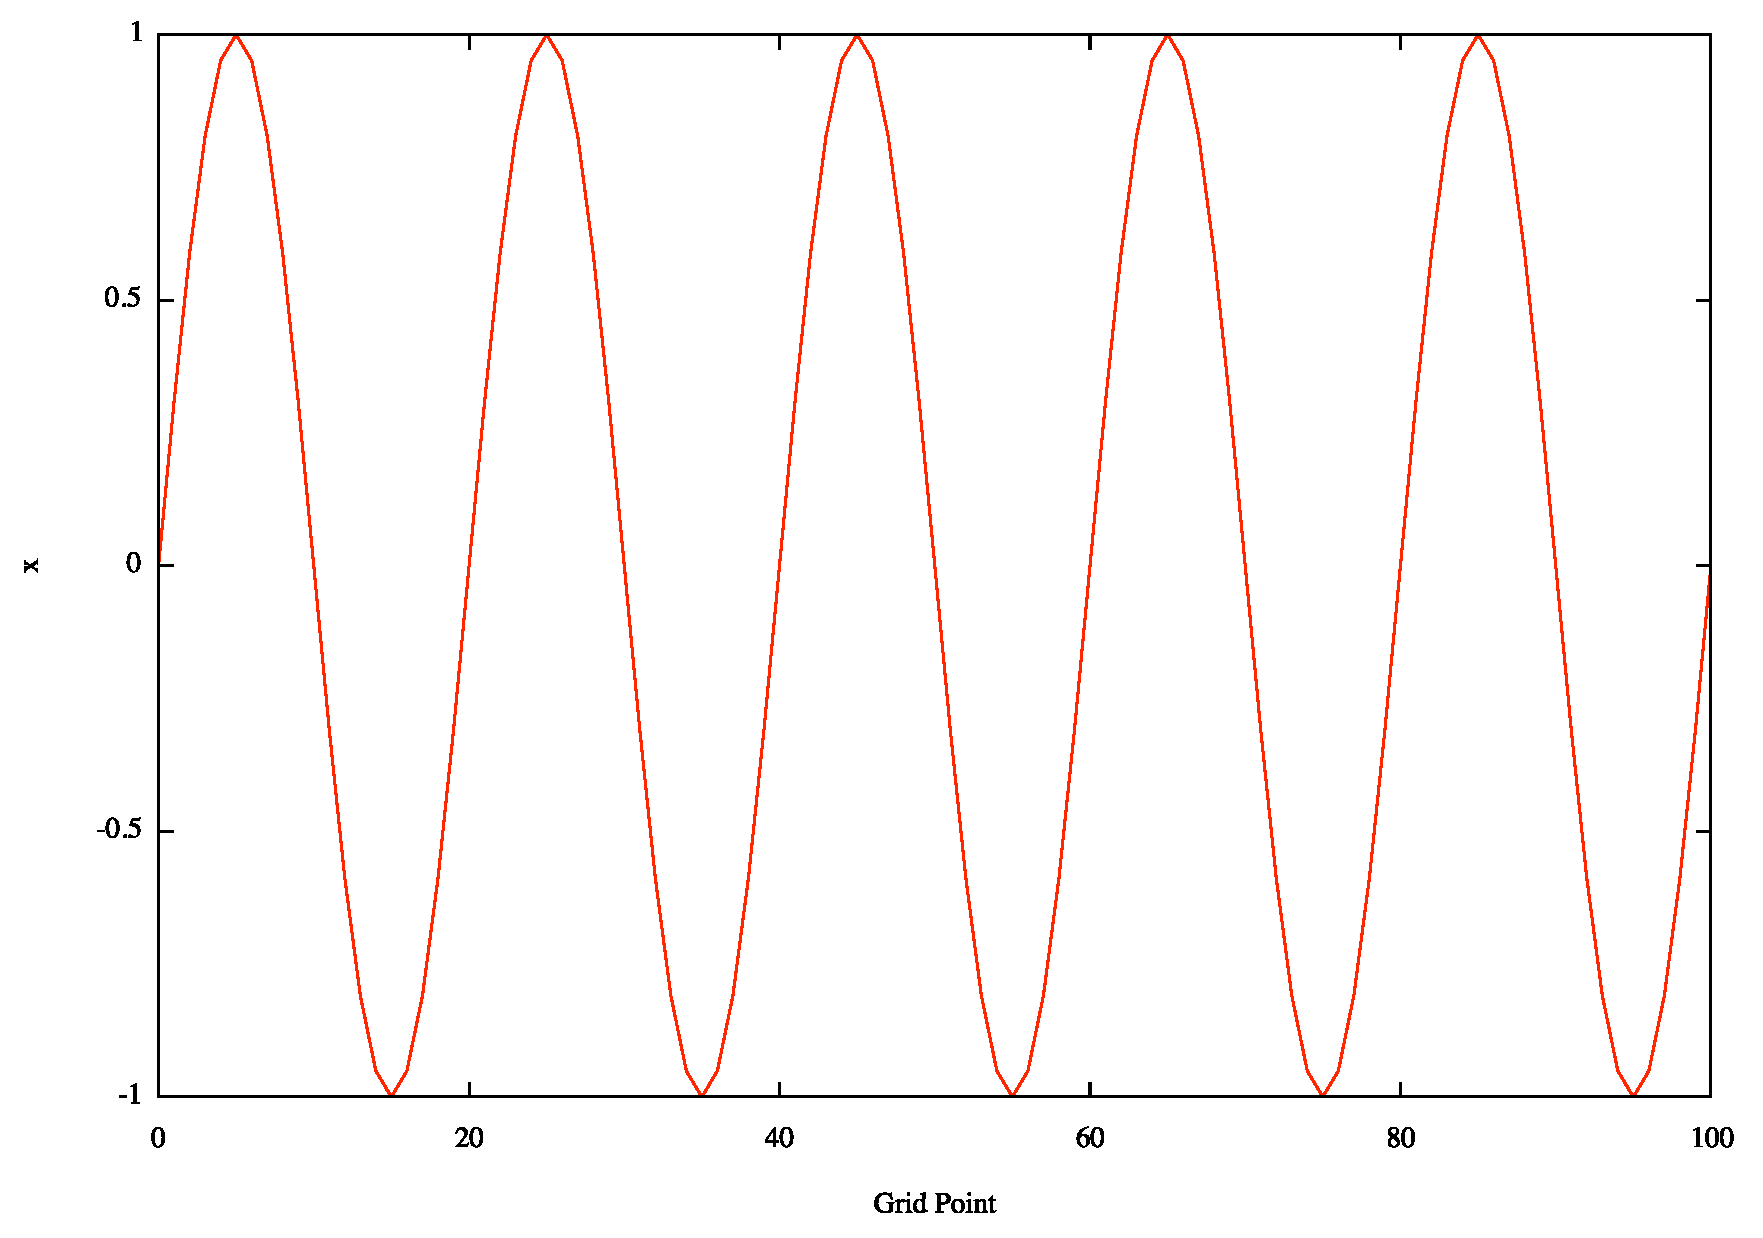
\includegraphics[width=1.5in]{mode_10.pdf}
        \caption{\textbf{$k = 10$.}}
      \end{figure}

    \end{column}

    \begin{column}{0.7\textwidth}

      \vspace{-0.25in}

      { \tiny
        \begin{table}[h!]
          \begin{center}
            \begin{tabular}{cc}\hline\hline
              \multicolumn{1}{c}{\textbf{Wave Number}} & 
              \multicolumn{1}{c}{\textbf{Time per History (s)}} \\
              \hline
              1 & 1 \\
              5 & 0.85 \\
              10 & 0.83 \\
              \hline\hline
            \end{tabular}
          \end{center}
          \caption{\textbf{Normalized average time per history.}}
          \label{tab:mc_timing}
        \end{table}
      }

      \vspace{-0.25in}

      \begin{itemize}
      \item $\sigma(A)$ dictates the characteristics of the Markov
        chain
        \smallskip
      \item Random walks are shorter for larger $k$
        \smallskip
      \item $N$ dictates the convergence of the Monte Carlo method
        \smallskip
      \item More samples required to resolve fine structures
      \end{itemize}

    \end{column}

  \end{columns}

\end{frame}

%%---------------------------------------------------------------------------%%
\begin{frame}{Multilevel Monte Carlo Methods}

  \begin{itemize}
  \item Formalized for integral equations (Heinrich,2001)
    \medskip
  \item Expanded for time-dependent finance calculations (Giles,2008)
    \medskip
  \item Recent work includes techniques for stochastic elliptic PDEs
    in ground water flow (Cliffe,2011) (Teckentrup,2013)
    \medskip
  \item Idea is to leverage multigrid ideas to reduce variance
  \end{itemize}

\end{frame}

%%---------------------------------------------------------------------------%%
\begin{frame}{Multilevel Expectation}

  Start first with the standard Monte Carlo estimator for the
  solution vector:
  \[
  \hat{\ve{x}} = \frac{1}{N} \sum_{m=1}^N x^m
  \]

  \medskip

  Consider $L$ levels with level 0 the finest $L$ the coarsest:
  \[
  E(\ve{x}_{0}) = E(\ve{x}_{L}) + E(\ve{x}_{L-1} - \ve{x}_{L}) +
  E(\ve{x}_{L-2} - \ve{x}_{L-1}) + \dots + E(\ve{x}_{0} - \ve{x}_{1})
  \]

  \medskip

  Reduce to a sum:
  \[
  \hat{\ve{y}}_{l} = \frac{1}{N_l} \sum_{m=1}^{N_l} (x^m_{l} -
  x^m_{l+1})
  \]

\end{frame}

%%---------------------------------------------------------------------------%%
\begin{frame}{Multilevel Expectation}

  Build a correction estimator for a given level $l$:
  \[
  \hat{\ve{y}}_{l} = \frac{1}{N_l} \sum_{m=1}^{N_l} (x^m_{l} -
  x^m_{l+1})
  \]

  \medskip

  Leaving a final multilevel estimator of:
  \[
  \hat{\ve{x}} = \sum_{l=0}^L \hat{\ve{y}}_{l}
  \]

  \medskip

  \textbf{Critical observation:} $x^m_{l}$ and $x^m_{l+1}$
  must be constructed from the \textit{same} Markov chain

\end{frame}

%%---------------------------------------------------------------------------%%
\begin{frame}{Constructing Multilevel Estimates}

  Define a \textit{prolongation operator}, $\ve{P}_l$, and a
  \textit{restriction operator}, $\ve{R}_l$, with variational conditions:
  \[
  \ve{R} = c \ve{P}^T
  \]
  \[
  \ve{A}_{l+1} = \ve{R}_l\ve{A}_l\ve{P}_l
  \]

  Use to build the multilevel estimate:
  \[
  E(\ve{x}_{l} - \ve{x}_{l+1}) = \Big(\ve{I} - \ve{P}_l \ve{R}_l\Big)
  \hat{\ve{x}}_{l}
  \]
  where $\hat{\ve{x}}_{l}$ is constructed from the standard adjoint
  estimator at level $l$

  \medskip
  
  Number of samples at each level should be determined from the
  estimated variance. For simplicity (Heinrich,2001):
  \[
  N_l = M^{-3(L-l)/2}N
  \]

\end{frame}

%%---------------------------------------------------------------------------%%
\begin{frame}[fragile]{Multilevel Monte Carlo Solver}
  
  \vspace{-0.15in}

  \begin{algorithm}[H]
    \caption{\small Multilevel Monte Carlo Method}
    \label{alg:mlamc}
    \begin{algorithmic}[1]
      { \small
        \FOR{ l = 0...L }
        \STATE  $\ve{P}_l = P(\ve{A}_l)$
        \COMMENT{Build the prolongation and restriction operators for
          the $l^{th}$ level.}
        \STATE $\ve{R}_l = c \ve{P}_l^T$
        \STATE $\ve{r}_l = \ve{b}_l - \ve{A}_l \ve{x}_l^0$
        \COMMENT{Build the $l^{th}$ level residual.}
        \STATE $\ve{d}_l = \hat{\ve{A}}_l^{-1} \ve{r}_l$
        \COMMENT{Solve the $l^{th}$ level problem with adjoint Monte
          Carlo}
        \IF{ l != L }
        \STATE $\ve{d}_l = (\ve{I} - \ve{P}_l\ve{R}_l) \ve{d}_{l}$
        \COMMENT{Apply the multilevel tally}
        \STATE $\ve{A}_{l+1} = \ve{R}_l \ve{A}_l \ve{P}_l$
        \COMMENT{Construct the next level.}
        \STATE $\ve{x}_{l+1}^0 = \ve{R}_l \ve{x}_l^0$
        \STATE $\ve{b}_{l+1} = \ve{R}_l \ve{b}_l$
        \ENDIF
        \ENDFOR

        \FOR{ l = L...1 }
        \STATE $\ve{d}_{l-1} = \ve{d}_{l-1} + \ve{P}_{l} \ve{d}_{l}$
        \COMMENT{Collapse the tallies to the finest grid}
        \ENDFOR
        \STATE $\ve{x} = \ve{x}^0 + \ve{d}_0$
      }
    \end{algorithmic}
  \end{algorithm}

\end{frame}

%%---------------------------------------------------------------------------%%
\begin{frame}{Numerical Experiments}

  \begin{itemize}
  \item Solve the model problem on grid size 1024 and $N = 10,000$
    \medskip
  \item Geometric multigrid operators from Briggs' multigrid tutorial,
    $M = 2$
    \medskip
  \item Algebraic multigrid operators from ML, $M \approx 3$
  \end{itemize}

  \bigskip
  Measure performance with a \textit{figure of merit}:
  \[
  FOM = \frac{1}{||\ve{e}||^2_{\infty} T}
  \]

\end{frame}

%%---------------------------------------------------------------------------%%
\begin{frame}{Geometric Multigrid Results}

  \begin{columns}

    \begin{column}{0.5\textwidth}

      { \tiny
        \begin{table}[h!]
          \begin{center}
            \begin{tabular}{cllll}\hline\hline
              \multicolumn{1}{c}{\textbf{Levels}} & 
              \multicolumn{1}{l}{\textbf{Samples}} & 
              \multicolumn{1}{l}{\textbf{$||\ve{e}||_{\infty}$}} & 
              \multicolumn{1}{l}{\textbf{Time (s)}} & 
              \multicolumn{1}{l}{\textbf{RFOM}} \\
              \hline
              1 & 10,000 & 0.022 & 119.1 & 1 \\
              2 & 13,535 & 0.026 & 72.0 & 1.14 \\
              3 & 14,785 & 0.035 & 33.2 & 1.38 \\
              4 & 15,226 & 0.039 & 13.7 & 2.63 \\
              5 & 15,382 & 0.027 & 5.5 & 13.86 \\
              6 & 15,437 & 0.036 & 2.3 & 19.21 \\
              7 & 15,456 & 0.045 & 0.98 & 28.00 \\
              8 & 15,462 & 0.081 & 0.41 & 20.66 \\
              9 & 15,464 & 0.267 & 0.17 & 11.72 \\
              \hline\hline
            \end{tabular}
          \end{center}
          \caption{\textbf{$k = 1$.}}
          \label{tab:k1_results}
        \end{table}
      }

      \vspace{-0.25in}

      { \tiny
        \begin{table}[h!]
          \begin{center}
            \begin{tabular}{cllll}\hline\hline
              \multicolumn{1}{c}{\textbf{Levels}} & 
              \multicolumn{1}{l}{\textbf{Samples}} & 
              \multicolumn{1}{l}{\textbf{$||\ve{e}||_{\infty}$}} & 
              \multicolumn{1}{l}{\textbf{Time (s)}} & 
              \multicolumn{1}{l}{\textbf{RFOM}} \\
              \hline
              1 & 10,000 & 0.668 & 101.6 & 1 \\
              2 & 13,535 & 0.381 & 60.0 & 5.21 \\
              3 & 14,785 & 0.396 & 28.0 & 10.34 \\
              4 & 15,226 & 0.599 & 11.9 & 10.64 \\
              5 & 15,382 & 0.638 & 4.7 & 23.60 \\
              6 & 15,437 & 1.052 & 1.8 & 23.15 \\
              7 & 15,456 & 1.070 & 0.67 & 59.16 \\
              8 & 15,462 & 1.180 & 0.23 & 144.10 \\
              9 & 15,464 & 2.130 & 0.10 & 99.95 \\
              \hline\hline
            \end{tabular}
          \end{center}
          \caption{\textbf{$k = 5$.}}
          \label{tab:k5_results}
        \end{table}
      }

    \end{column}

    \begin{column}{0.5\textwidth}

      { \tiny
        \begin{table}[h!]
          \begin{center}
            \begin{tabular}{cllll}\hline\hline
              \multicolumn{1}{c}{\textbf{Levels}} & 
              \multicolumn{1}{l}{\textbf{Samples}} & 
              \multicolumn{1}{l}{\textbf{$||\ve{e}||_{\infty}$}} & 
              \multicolumn{1}{l}{\textbf{Time (s)}} & 
              \multicolumn{1}{l}{\textbf{RFOM}} \\
              \hline
              1 & 10,000 & 1.81 & 98.6 & 1 \\
              2 & 13,535 & 1.67 & 59.6 & 1.94 \\
              3 & 14,785 & 2.41 & 27.1 & 2.05 \\
              4 & 15,226 & 3.20 & 11.5 & 2.74 \\
              5 & 15,382 & 1.85 & 4.93 & 19.14 \\
              6 & 15,437 & 3.89 & 1.95 & 10.95 \\
              7 & 15,456 & 3.79 & 0.78 & 28.68 \\
              8 & 15,462 & 7.08 & 0.30 & 21.62 \\
              9 & 15,464 & 11.7 & 0.11 & 21.45 \\
              \hline\hline
            \end{tabular}
          \end{center}
          \caption{\textbf{$k = 10$.}}
          \label{tab:k10_results}
        \end{table}
      }

      \vspace{-0.25in}

      \begin{itemize}
      \item There is a limit to the number of levels
      \item Too few samples on the fine grid drive up the error
      \end{itemize}

    \end{column}

  \end{columns}

\end{frame}

%%---------------------------------------------------------------------------%%
\begin{frame}{Algebraic Multigrid Results}

  \begin{columns}

    \begin{column}{0.5\textwidth}

      { \tiny
        \begin{table}[h!]
          \begin{center}
            \begin{tabular}{cllll}\hline\hline
              \multicolumn{1}{c}{\textbf{Levels}} & 
              \multicolumn{1}{l}{\textbf{Samples}} & 
              \multicolumn{1}{l}{\textbf{$||\ve{e}||_{\infty}$}} & 
              \multicolumn{1}{l}{\textbf{Time (s)}} & 
              \multicolumn{1}{l}{\textbf{RFOM}} \\
              \hline
              1 & 10,000 & 0.022 & 119.1 & 1 \\
              2 & 11,924 & 0.037 & 31.9 & 1.28 \\
              3 & 12,294 & 0.055 & 7.6 & 2.40 \\
              4 & 12,365 & 0.051 & 1.8 & 11.76 \\
              5 & 12,378 & 0.094 & 0.5 & 12.01 \\
              \hline\hline
            \end{tabular}
          \end{center}
          \caption{\textbf{$k = 1$.}}
          \label{tab:ml_k1_results}
        \end{table}
      }

      \vspace{-0.25in}

      { \tiny
        \begin{table}[h!]
          \begin{center}
            \begin{tabular}{cllll}\hline\hline
              \multicolumn{1}{c}{\textbf{Levels}} & 
              \multicolumn{1}{l}{\textbf{Samples}} & 
              \multicolumn{1}{l}{\textbf{$||\ve{e}||_{\infty}$}} & 
              \multicolumn{1}{l}{\textbf{Time (s)}} & 
              \multicolumn{1}{l}{\textbf{RFOM}} \\
              \hline
              1 & 10,000 & 0.668 & 101.6 & 1 \\
              2 & 11,924 & 0.834 & 30.8 & 2.12 \\
              3 & 12,294 & 1.140 & 7.5 & 4.63 \\
              4 & 12,365 & 0.975 & 1.6 & 29.09 \\
              5 & 12,378 & 2.240 & 0.4 & 25.10 \\
              \hline\hline
            \end{tabular}
          \end{center}
          \caption{\textbf{$k = 5$.}}
          \label{tab:ml_k5_results}
        \end{table}
      }

    \end{column}

    \begin{column}{0.5\textwidth}

      { \tiny
        \begin{table}[h!]
          \begin{center}
            \begin{tabular}{cllll}\hline\hline
              \multicolumn{1}{c}{\textbf{Levels}} & 
              \multicolumn{1}{l}{\textbf{Samples}} & 
              \multicolumn{1}{l}{\textbf{$||\ve{e}||_{\infty}$}} & 
              \multicolumn{1}{l}{\textbf{Time (s)}} & 
              \multicolumn{1}{l}{\textbf{RFOM}} \\
              \hline
              1 & 10,000 & 1.81 & 98.6 & 1 \\
              2 & 11,924 & 2.33 & 30.0 & 1.99 \\
              3 & 12,294 & 3.19 & 7.6 & 4.20 \\
              4 & 12,365 & 3.31 & 1.8 & 16.29 \\
              5 & 12,378 & 9.98 & 0.5 & 7.21 \\
              \hline\hline
            \end{tabular}
          \end{center}
          \caption{\textbf{$k = 10$.}}
          \label{tab:ml_k10_results}
        \end{table}
      }

      \vspace{-0.25in}

      \begin{itemize}
      \item Algebraic operators are also effective
      \item $M \approx 3$ is an ad hoc estimate - need variance
        estimates instead
      \end{itemize}

    \end{column}

  \end{columns}

\end{frame}

%%---------------------------------------------------------------------------%%
\begin{frame}{Summary}

  \begin{itemize}
    \item Multilevel Monte Carlo methods can be an effective variance
      reduction technique by reducing the computation time needed to
      reach a particular error
      \medskip
    \item More formal analysis of convergence in the context of linear
      systems is required
      \medskip
    \item For large problems, density of $A_l$ for coarse levels
      increases computational complexity of the Monte Carlo - consider
      non-Galerkin and sparsification approaches
      \medskip
    \item Future work includes addition of variance estimation to
      properly select $N_l$
  \end{itemize}

\end{frame}

%%---------------------------------------------------------------------------%%
\begin{frame}{Acknowledgments}

  This work was sponsored by the U.S. Department of Energy Office of
  Advanced Scientific Computing Research (ASCR). \textit{MCREX: Using
    Monte Carlo algorithms to achieve resiliency and performance at
    scale for linear and non-linear solver applications}

  \bigskip
  \bigskip
  
  This work has been authored by UT-Battelle, LLC, under contract
  DE-AC05-00OR22725 with the U.S. Department of Energy.

\end{frame}

%%---------------------------------------------------------------------------%%

\end{document}
